\lecture{9}{31.07.2020}{Kalman Filter and LQG Control}

With the observer, we wanted to place the poles to balance uncertainty and knowledge in the measure and uncertainty and knowledge in the model, but we had no quantitative representation of uncertainty. With the random process described as a Gaussian random process we describe the uncertainty through the mean and the variance. We also can, now, describe the effect of a deterministic system in this gaussian domain.

Define a system defined by \[
    \dot{x}(t)=Ax(t) + B_uu(t) + B_ww(t)
\] \[
m(t) = C_mx(t) + v(t)
\], where $w(t)$ is the noise input of the system and $v(t)$ is the measurement noise. Note that we also replace $y(t)$ by $m(t)$ to represent better the idea we are modelling the mean value of the output. This way we now model our system with \emph{white noise}, that is \[
E\left[ w(t)w^{T}(t+\tau) \right] = S_w\delta(\tau)
\] \[
E\left[ v(t)v^{T}(t+\tau) \right] = S_v\delta(\tau)
\] defines the noises covariance. Furthermore, we assume 
\begin{equation*}
    \begin{split}
& E\left[ v(t)w^{T}(t+\tau) \right] = 0 \\
& E\left[ x(t)w^{T}(t+\tau) \right] = 0 \\
& E\left[ x(t)v^{T}(t+\tau) \right] = 0
    \end{split}
\end{equation*}
that is: the noises are not correlated; the input noise is not correlated to the initial conditions; and the measurement noise is not correlated to the state.o

Now  the Kalman filter has the objective to minimize the mean square estimation error \[
    J=E\left[ \left\{ x(t)-\hat{x}(t) \right\}^{T}\left\{ x(t)-\hat{x}(t) \right\}   \right] 
\] at \textbf{each instant}. Note that the expression within the brackets is the difference between the model results and the measurements of the state, and thus we are minimizing the expected value of the square of the module (inner product) of this difference.

The model is given by \[
    \dot{\hat{x}}(t)=A(t)\hat{x}(t)+B_uu(t) +G(t)\left[ m(t)-C_m\hat{x}(t) \right] 
\] where $G(t)$ is the Kalman Gain matrix of the filter. Notice that it is very similar to the observer model previously defined, with the exception that the gain matrix is \emph{time varying}.

The Kalman Gain is obtained through the orthogonality condition. It can be demonstrated that the gain can be defined analytically by \[
G(t)=\Sigma_e(t)C_m^{T}S_v^{-1}
\] .

Note that, now, the Kalman Filter observer is a \textbf{time varying system}, so not possible anymore to deal with eigenvalues.

Also, it is of interest to look at the dynamic of the error \[
    \dot{e}(t)=\dot{x}(t)-\dot{\hat{x}}(t)
\] which develops in \[
\dot{e}(t)=\left[ A-G(t)C_m \right] e(t) + \left[ B_w-G(t) \right] \begin{bmatrix} w(t) \\ v(t) \end{bmatrix} 
\]. So we see the first part very similar to the classical observer and the second part the relation to the noise in the system.

Through the Riccati equation of the error we can find the dynamic of the covariance matrix of the estimation error as \[
\dot{\Sigma_e}(t)=\Sigma_e(t)A^{T} + A\Sigma_e(t)+B_wS_wB_w^{T}-\Sigma_e(t)C_m^{T}S_v^{-1}C_m\Sigma_e(t)
\].

\subsection*{Summary}

The Kalman filter is defined by the following set of equations: \[
    \dot{\hat{x}}(t)=A(t)\hat{x}(t)+B_uu(t) +G(t)\left[ m(t)-C_m\hat{x}(t) \right]  \\
\] \[
G(t)=\Sigma_e(t)C_m^{T}S_v^{-1} \\
\] \[
\dot{\Sigma_e}(t)=\Sigma_e(t)A^{T} + A\Sigma_e(t)+B_wS_wB_w^{T}-\Sigma_e(t)C_m^{T}S_v^{-1}C_m\Sigma_e(t)
\] which are the \emph{observer equation}, the \emph{gain equation}, and the \emph{covariance equation}. In time domain, this is happening all together, but one can imagine the steps as doing the prediction (first two terms of the observer equation), update the covariance, calculate the gain and, finally the correction (third term of the observer equation).

As an exercise, imagine that the uncertainty of the measurement $S_v$ goes to 0, then the gain $G(t)$ goes to infinity and the update of the state $\dot{\hat{x}}$ weights towards the measurement. If otherwise, $S_v \to \infty$, then $G(t)\to 0$ and, therefore, the update of the states will trust the model only.

\subsection*{Steady-State Kalman Filter}

Similarly to the LQR. One can show that after a transient, the Kalman Filter reaches a steady-state value, so the steady-state KF assumes the steady-state values from the beginning. It can be calculated through the Hamiltonian, the Riccati, by setting $\dot{\Sigma_e}(t)=0 $.

\subsection*{LQG Control}

Combines LQR and the Kalman Filter. The model is described by the formulation of the KF as \[
    \dot{x}(t)=Ax(t) + B_uu(t) + B_ww(t)
\] \[
m(t) = C_mx(t) + v(t)
\] adding \[
y(t)=C_yx(t)
\], with the same assumptions (uncorrelated white noises).

Now we define the cost function as \[
    J(y(t),u(t))=E\left[ \frac{1}{2}y^{T}(t_f)H_yy(t_f) + \frac{1}{2}\int_0^{t_f}\left\{ y^{T}(t)Q_yy(t)+u^{T}(t)Ru(t) \right\} dt \right] 
\]. Note that we have as well the case where $t_f\to \infty$, which will result the steady-state LQR and KF.

\begin{figure}[h]
    \centering
    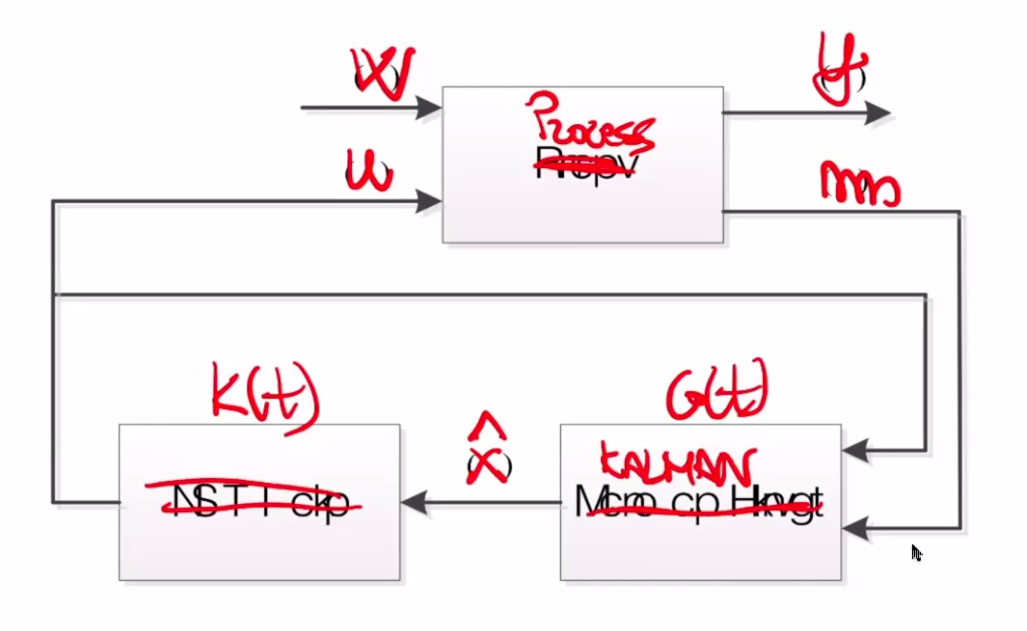
\includegraphics[width=0.8\textwidth]{figures/LQG_diagram.png}
    \caption{LQG diagram. $K(t)$ is on the LQR block}
    \label{fig:LQG-diagram}
\end{figure}

So the controller will be calculated upon the KF estimation, that is, \[
u(t)=-K(t)\hat{x}(t)
\] . All the rest remains the same, gain calculation, model equations, covariance matrix, initial conditions, etc. Note that \textbf{the design of the filter and of the controller can be done separately}.

\subsection*{Discrete Kalman Filter}

Given the complexity of the systems, it is very difficult to implement through analog control. So we will reformulate the approach in the discrete domain.

For $k$ measurements $y$, modeled as dependent from a variable $x$ that needs to be estimated, we have the following formulation in the presence of noise $v$: \[
    \begin{bmatrix} y_1\\ \vdots\\ y_k \end{bmatrix}=\begin{bmatrix} h_{11} & \ldots & h_{1n} \\ \vdots & \ddots & \vdots \\ h_{k_1} & \ldots & h_{kn} \end{bmatrix} \begin{bmatrix} x_1\\ \vdots\\ x_n \end{bmatrix}
\] \[
y=Hx+v
\], that is, $y$ depends differently over time on the values of $x$. Defining a cost function as the square of the error (inner product), one can define the ideal least-squares estimator as \[
\hat{x}=\left( H^{T}H \right) ^{-1}H^{T}y
\] .

Note that we are dealing with the situation where \[
x_{k+1} = x_k
\] for demonstration purposes.

To introduce confidence in the measurement, assuming that the noise has mean zero and is independent, one defines the following matrix upon the standard deviations of the measurement \[
R = E\left[ vv^{T} \right] 
\] which is added to the cost function and implies in a new estimator \[
\hat{x}=\left( H^{T}R^{-1}H \right) ^{-1}H^{T}R^{-1}y
\] .

Now, if the measurements are obtained in a sequential manner, the above equation is applied at each time, which implies in growing $H$ and $R$, so we achieve an recursive equation for the estimations, that is, given estimate $\hat{x}_{k-1}$ after $k-1$ measurements, one wants to determine $\hat{x}_k$ to determine $y_k$.

The recursive structure now is
\begin{equation}\label{x_k_equation}
    \hat{x}_k=\hat{x}_{k-1}+K_k\left( y_k-H_k\hat{x}_k-1 \right) 
\end{equation}
where $K_k$ is the estimator gain matrix and is multiplied by the correction term.

Using the sum of the squares of error variances as the objective function, we can calculate the covariance matrix as
\begin{equation}\label{P_k_equation}
    P_k = \left( I-K_kH_k \right) P_{k-1}\left( I-K_kH_k \right)^{T} + K_kR_kK_k^{T}
\end{equation}
and the optimal gain matrix through
\begin{equation}\label{K_k_equation}
    K_k=P_{k-1}H_k^{T}\left( H_kP_{k-1}H_k^{T}+R_k \right) ^{-1}
\end{equation}
and run the filter as

INSERT ALGORITHM

\begin{enumerate}
    \item For $k=0$, initialise a guess for $\hat{x}_0 and P_0$
    \item For $k=1,2,3,\ldots$
	\begin{enumerate}
	    \item Calculate $K_k$ given (\ref{K_k_equation})
	    \item Update $\hat{x}_{k-1}$ with the new measurement $y_k$ given equation (\ref{x_k_equation})
	    \item Update $P_k$ using equation (\ref{P_k_equation})
	\end{enumerate}
\end{enumerate}

With this, we end up, in a way, cleaning a measurement with noise. Another application is in the situation where the noise has a broad range of frequencies and a low-pass filter would interfere with the frequencies of the controller.

Now, in a deterministic but uncertain model, we model the expected value and covariance, and again we see that the mean is propagated through the system dynamic as with the model without uncertainty. On the other hand, the covariance is propagated following \[
P_k = F_{k-1}P_{k-1}F_{k-1}^{T} + Q_{k-1}
\]. With these, we can now understand the application of the Kalman filter as in the figure below.

\begin{figure}[h]
    \centering
    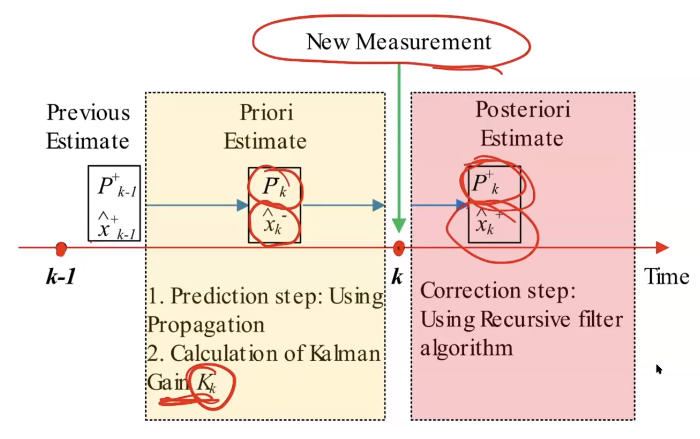
\includegraphics[width=0.8\textwidth]{figures/kalman_filter_prediction.png}
    \caption{Kalman Filter prediction diagram.}
    \label{fig:kalman_filter_prediction}
\end{figure}

So our estimate of the state expected value as \[
\hat{x}_k^+ = \hat{x}_k^- + K_k\left( y_k - H\hat{x}_k^- \right) 
\] and covariance would be \[
P_k^+ = \left( I - K_kH \right) P_k^- \left( I-K_kH \right)^{T} + K_kRK_k^{T}
\].

\textbf{Note on steady-state approach}

The usefulness of the steady-state version of both Kalman filter and LQR is defined by the duration of the transient of the system's characteristics that affect the model. So if the transient of the Kalman gain lasts a few seconds and the application is run for hours, than it is probably not worth it to use the time-variant version of it.
